\documentclass[dvipdfmx, 9pt, a4paper]{jsarticle}
\usepackage[margin=15mm]{geometry}
\usepackage{fancyhdr}
\usepackage{multirow}
\usepackage{amsmath,  amssymb}
\usepackage{type1cm}
\usepackage{latexsym}
\usepackage{algorithmic}
\usepackage{algorithm}
\usepackage{ascmac}
\usepackage{listings,jvlisting}
\usepackage{tcolorbox}
\usepackage[utf8]{inputenc}
\usepackage{color}

\DeclareFixedFont{\ttb}{T1}{txtt}{bx}{n}{9}
\DeclareFixedFont{\ttm}{T1}{txtt}{m}{n}{9}
\definecolor{deepblue}{rgb}{0,0,0.5}
\definecolor{deepred}{rgb}{0.6,0,0}
\definecolor{deepgreen}{rgb}{0,0.5,0}

\renewcommand{\theequation}{\arabic{section}.\arabic{equation}}
\renewcommand{\thefigure}{\arabic{section}.\arabic{figure}}
\renewcommand{\thetable}{\arabic{section}.\arabic{table}}
\makeatletter
\@addtoreset{equation}{section}
\@addtoreset{figure}{section}
\@addtoreset{table}{section}
\AtBeginDocument{
  \renewcommand*{\thelstlisting}{\arabic{section}.\arabic{lstlisting}}%
  \@addtoreset{lstlisting}{section}
}

\numberwithin{equation}{section}

\renewcommand{\baselinestretch}{0.78}
\newcommand{\bm}[1]{{\mbox{\boldmath $#1$}}}
\newcommand{\bnabla}{\bm \nabla}
\newtheorem{Proof}{証明}
\def\qed{\hfill $\Box$}

\lstset{language=Fortran,%
        basicstyle=\footnotesize,%
        commentstyle=\textit,%
        classoffset=1,%
        keywordstyle=\bfseries,%
	frame=tRBl,framesep=5pt,%
	showstringspaces=false,%
        numbers=left,stepnumber=1,numberstyle=\footnotesize%
	}%


\begin{document}
\begin{center}
{\fontsize{18pt}{1pt}\selectfont 最適化手法}\\
\end{center}

\section{勾配による実数値最適化}
\subsection{前準備}
本章では多次元の実数値最適化を扱う。また、最適化の対象である数値のことを解、またはパラメータと呼び、$\bm x$のように書き表す。解が取り得る集合を$V$とする。問題が制約なし最適化の場合、$V=\mathbb{R}^n$となる($n$は解の次元)。本資料では一貫して、目的関数$f:V \to \mathbb{R}$の最小化が最適化だと考える。従って問題は${\rm min}_{\bm x \in V} f(\bm x)$と定式化される。\par
$\bm x^* \in V$が任意の$\bm x \in V$に対して$f(\bm x^*) \leq f(\bm x)$となるとき、$\bm x^*$のことを{\bf 大域的最適解}と呼ぶ。この$\bm x^*$こそ私たちの知りたい値であり、最適化手法に要求する値である。しかしながら、世の手法のほとんどは大域的最適解の出力を保証してくれない。あくまで保証してくれるのは、「適切なハイパーパラメータの基で十分に計算したときに局所最適値に収束する」ことだけである。いま、$\bm x$の$\epsilon$近傍$B$を
\begin{equation}
B(\bm x, \epsilon)=\{ \bm y \in V||| \bm x-\bm y || < \epsilon \}
\end{equation}
と定義する。ある解$\bm x^*$と任意の解$\bm x \in B(\bm x^*, \epsilon) \cap V$に対して、$f(\bm x^*) \leq f(\bm x)$が成り立つとき、$\bm x^*$のことを{\bf 局所最適解}と言う。従って如何なる最適化手法も、周囲と比べて適した解を提供してくれるに過ぎない(それでも十分嬉しかったりする)。

\subsubsection{局所最適解の特徴}
\begin{itembox}[l]{定理1.1.1(1次の必要条件)}
 $\bm x^*$が局所最適解であるとき、$\bnabla f(\bm x^*)=\bm 0$が成立する。
\end{itembox}
{\bf 証明}:任意のベクトル$\bm \delta$と正の非常に小さいスカラー$t$を考える。このとき局所最適解の条件より、$f(\bm x^*+t\bm \delta)-f(\bm x^*) \geq 0$が成立する。そこで$t \to +0$としたとき、テイラー展開より$\bm \nabla f(\bm x^*)\cdot \bm \delta$が成立する。これは$\bm \delta=-\bm \nabla f(\bm x^*)$でも成り立つので、$-\bm \nabla f(\bm x^*)\cdot \bm \nabla f(\bm x^*) \geq 0$となるが、内積の定義より、$\bm \nabla f(\bm x^*)=\bm 0$が得られる。\qed \par
$\bm \nabla f(\bm x)=\bm 0$となるような点を{\bf 停留点}と言う。停留点であることは局所最適値である十分条件ではない。例えば関数の極大値は停留点であるが局所最適値ではない。\par
次に2次の必要条件を考えるが、本資料ではヘッセ行列$\bm \nabla(\bm \nabla f(\bm x))$を$\bm \nabla^2f(\bm x)$のように書く(なお、前者の書き方はダイアディクの定義に従う)。
\begin{itembox}[l]{定理1.1.2(2次の必要条件)}
 $\bm x^*$が局所最適解であるとき、ヘッセ行列$\bm \nabla^2f(\bm x^*)$は半正定値行列となる。
\end{itembox}
{\bf 証明}:任意のベクトル$\bm \delta$と正の非常に小さいスカラー$t$を考える。$t \to +0$としたとき、$f(\bm x^*+t\bm \delta)-f(\bm x^*) \geq 0$が成立する。先ほど同様テイラー展開を施し、$\bm \nabla f(\bm x^*)=\bm 0$を考慮すれば、$\bm \delta \cdot (\bm \nabla^2f(\bm x^*)\bm \delta) \geq 0$なる関係が得られる。\qed
\begin{itembox}[l]{定理1.1.3(2次の十分条件)}
 $\bm x^* \in V$に対して、$\bm \nabla f(\bm x^*)=\bm 0$かつ$\bm \nabla^2f(\bm x^*)$が半正定値行列であるとき、$\bm x^*$は局所最適値である。
\end{itembox}
\subsubsection{最適化手法の停止条件}
定理1.3より、最適化手法は勾配がゼロでヘッセ行列が半正定値行列となるような$\bm x^*$を目指す。しかしながら数値計算的上、厳密に勾配がゼロとなるような点に収束することは難しいので、別途アルゴリズムの停止条件は必要である。\par
考えられる停止条件として最も単純なものは
\begin{equation}
|| \bm \nabla f(\bm x) || < \epsilon \notag
\end{equation}
であろう。ここで$\epsilon$はハイパーパラメータであるが、浮動小数点の誤差を考慮して$10^{-16}$を採用することが比較的多い。\par
しかしながら、これは目的関数の出力のオーダーに依存する。例えば$f$が何か物理量を出力する場合、採用したSI単位によって$f$の値は変わるが、それによって停止条件の"厳しさ"も変わるのは、ときに好ましくない。この対策として
\begin{equation}
|| \bm \nabla f(\bm x) || < \epsilon|f(\bm x)| \notag
\end{equation}
なる停止条件も提案された。ただし、これは$|f(\bm x)|$の値が非常に小さいときに厳しすぎる停止条件となるので、代わりに
\begin{equation}
|| \bm \nabla f(\bm x) || < \epsilon(1+|f(\bm x)|) \notag
\end{equation}
を採用することもある。今では、下記の条件がすべて満たされたときに停止させることが多い。各停止条件を判定するFortranの関数を以下に示す。
\begin{lstlisting}[caption=停止条件]
function stop_condition1(gradf, epsilon) result(cond)
	implicit none
	real, intent(in) :: gradf(:)
	real, optional, intent(in) :: epsilon
	logical :: cond
	real :: norm_gradf
	norm_gradf = sqrt(sum(gradf**2))

	if (present(epsilon)) then
		cond = (norm_gradf < epsilon)
	else
		cond = (norm_gradf < 1.0e-16)
	end if
	return
end function stop_condition1

function stop_condition2(gradf, f, epsilon) result(cond)
	implicit none
	real, intent(in) :: gradf(:), f
	real, optional, intent(in) :: epsilon
	logical :: cond
	real :: norm_gradf
	norm_gradf = sqrt(sum(gradf**2))

	if (present(epsilon)) then
		cond = (norm_gradf < epsilon*abs(f))
	else
		cond = (norm_gradf < 1.0e-16*abs(f))
	end if

	return
end function stop_condition2

function stop_condition3(gradf, f, epsilon) result(cond)
	implicit none
	real, intent(in) :: gradf(:), f
	real, optional, intent(in) :: epsilon
	logical :: cond
	real :: norm_gradf
	norm_gradf = sqrt(sum(gradf**2))

	if (present(epsilon)) then
		cond = (norm_gradf < epsilon*(1. + abs(f)))
	else
		cond = (norm_gradf < 1.0e-16*(1. + abs(f)))
	end if

	return
end function stop_condition3
\end{lstlisting}

\subsection{最適化手法の紹介}
\subsubsection{最急降下法}
勾配を用いた最適化手法の中で最も単純なものは{\bf 最急降下法(SD法)}であろう。まず、解$\bm x \in V$と十分に小さいベクトル$\bm \delta(\bm x + \bm \delta \in V)$を考える。$f(\bm x+\bm \delta)$をテイラー展開し、第一項までを考慮したならば、
\begin{equation}
f(\bm x+\bm \delta) \simeq f(\bm x)+\bm \nabla f(\bm x)\cdot \bm \delta
\end{equation}
なる関係が得られる。SD法は解$\bm x$を$\bm x+\bm \delta$に更新し、それを繰り返すことで最終的に局所最適解に収束することを目指す。解の更新において式(1.2)は重要なヒントである訳だが、$\bm \delta$の大きさが小さいことを考えると、$f(\bm x+\bm \delta)$が最小となるのは、$\bm \delta$と$-\bnabla f(\bm x)$が同じ向きであるときだと分かる。従って、十分に小さい実数$\alpha$に対して$\bm \delta=-\alpha \bnabla f(\bm x)$とし、解を
\begin{equation}
\bm x \leftarrow \bm x-\alpha \bnabla f(\bm x)
\end{equation}
のように更新すればよい。以上がSD法における考え方である。\par
繰り返しになるが、式(1.2)の関係を仮定しているため、式(1.3)中の$\alpha$の値は十分に小さくなければならない。$\alpha$の値を決める方法として、数学的根拠のあるものがいくつか提案されているが、多くの場合は経験則的に決めてしまう。なお、$\alpha$のことを{\bf 緩和係数}というが、人工知能の分野では学習率と呼ぶことの方が多い。\par
緩和係数が適切に設定された場合、式(1.3)より解は勾配がゼロとなる点に収束する。したがって、SD法は関数の局所最適解ではなく停留点に収束することを保証する。この保証はいささか不十分に聞こえるかもしれないが、SD法が出力する停留点は局所最適解であることがほとんどなので、実用上の問題はない。\par
式(1.3)より、SD法はヘッセ行列を考えていないことが分かる。それゆえ局所最適解の収束を保証しなかった訳であるが、ヘッセ行列を考えない分だけ解の更新に要する計算コストが低いというメリットもある。それゆえSD法はいまでも利用されている。しかしながら、関数$f$によっては探索方向に問題があることも指摘されており、解の更新の計算コストが低いといっても解が収束するまでの時間が短いとは限らないことも事実である。

\begin{tcolorbox}[title = 最急降下法]
\begin{enumerate}
\item 初期解$\bm x_k \in \mathbb{R}^n$と$\alpha$を設定(ただし$k=0$)。
\item $\bm x_k$が停止条件を満たす場合、$\bm x_k$を出力して終了。
\item $\bm d_k \leftarrow -\alpha \bm \nabla f(\bm x_k)$。
\item $\bm x_{k+1} \leftarrow \bm x_k + \bm d_k$。
\item $k \leftarrow k+1$。ステップ2に戻る。
\end{enumerate}
\end{tcolorbox}\par
以下にSD法のFortranコード例(反復計算1回分)を示す。23行目でgradというサブルーチンを呼び出しているが、これは関数fの勾配をもとめるサブルーチンである(Listing1.3参照)。
\begin{lstlisting}[caption=SD法]
subroutine sd(f, x, alpha, hb)
	implicit none
	real, intent(in) :: alpha
	real, optional, intent(in) :: hb
	real, intent(inout) :: x(:)
	real :: h
	real :: df(size(x))

	interface
	function f(x)
		implicit none
		real, intent(in) :: x(:)
		real :: f
	end function f
	end interface

	if(present(hb)) then
		h = hb
	else
		h = 0.001
	end if

	call grad(f, x, df, h)

	x = x - alpha*df
	return
end subroutine sd
\end{lstlisting}

\begin{lstlisting}[caption=勾配計算のためのサブルーチン]
subroutine grad(f, x, df, hb)
	real, intent(in) :: x(:)
	real, optional, intent(in) :: hb
	real, intent(out) :: df(size(x))
	real :: dx(size(x)), h
	integer :: i
	interface
		function f(x)
			real, intent(in) :: x(:)
			real :: f
		end function f
	end interface

	if (present(hb)) then
		h = hb
	else
		h = 0.001
	end if

	i = 1
	do while(i <= size(x))
		dx = 0.; dx(i) = h
		df(i) = (f(x + dx) - f(x))/h
		i = i + 1
	end do

	return
end subroutine grad
\end{lstlisting}

\subsubsection{ニュートン法}
ニュートン法は最急降下法と違い、ヘッセ行列も加味する。2次の項まで加味したテイラー展開より、
\begin{equation}
f(\bm x+\bm \delta)\simeq f(\bm x)+\bm \nabla f(\bm x)\cdot \bm \delta + \frac{1}{2}\bm \delta \cdot (\bm \nabla^2f(\bm x)\bm \delta) \notag
\end{equation}
なる関係が得られる。最急降下法のときと同様、$f(\bm x+\bm \delta)$がより減少するような向き$\bm \delta$を知りたい。それは、上式を$\bm \delta$で微分した結果より、
\begin{equation}
\bm \delta = -(\bm \nabla^2 f(\bm x))^{-1}\bm \nabla f(\bm x) \notag
\end{equation}
だと分かる。ニュートン法ではこの向きに解を更新する。ただし、これはヘッセ行列が半正定値であることを仮定している。局所最適値付近では問題ないが、解の探索中は成り立たないこともある。そのようなとき、上式の更新方向は降下方向にならなかったりする。これはニュートン法の欠点であるため、修正された手法がいくつか提案されている。
\begin{tcolorbox}[title=ニュートン法]
\begin{enumerate}
\item 初期解$\bm x_k \in \mathbb{R}^n$と$\alpha$を設定(ただし$k=0$)。
\item $\bm x_k$が停止条件を満たす場合、$\bm x_k$を出力して終了。
\item $\bm d_k \leftarrow -\alpha(\bm \nabla^2 f(\bm x_k))^{-1}\bm \nabla f(\bm x_k)$。
\item $\bm x_{k+1} \leftarrow \bm x_k + \bm d_k$。
\item $k \leftarrow k+1$。ステップ2に戻る。
\end{enumerate}
\end{tcolorbox}\par
最急降下法のときもそうだが、関数の勾配やヘッセ行列は一般的に数値差分で求められる。そのため次元$n$が大きいとき、計算コストの面でヘッセ行列の数値計算には苦労する。多自由度な問題に対しニュートン法を利用することはお勧めしない。\par
以下はニュートン法のFortranコード例である。また、ヘッセ行列を計算するためのサブルーチンをListing1.5に記載した。
\begin{lstlisting}[caption=ニュートン法]
subroutine newton(f, x, alpha, hb)
	implicit none
	real, intent(in) :: alpha
	real, optional, intent(in) :: hb
	real, intent(inout) :: x(:)
	real :: h
	real :: ddf(size(x), size(x)), df(size(x))

	interface
	function f(x)
		implicit none
		real, intent(in) :: x(:)
		real :: f
	end function f
	end interface

	if(present(hb)) then
		h = hb
	else
		h = 0.001
	end if

	call hessian(f, x, ddf, h)
	call grad(f, x, df, h)

	x = x - alpha*matmul(ddf, df)
	return
end subroutine newton
\end{lstlisting}
\begin{lstlisting}[caption=ヘッセ行列を求めるためのサブルーチン]
subroutine hessian(f, x, ddf, hb)
	real, intent(in) :: x(:)
	real, optional, intent(in) :: hb
	real, intent(out) :: ddf(size(x), size(x))
	real :: h, df(size(x)), dx(size(x)), dfp(size(x))
	integer :: i, j

	interface
		function f(x)
			real, intent(in) :: x(:)
			real :: f
		end function f
	end interface

	if (present(hb)) then
		h = hb
	else
		h = 0.001
	end if

	i = 1
	do while(i <= size(x))
		call grad(f, x, df, h)

		j = 1
		do while(j <= size(x))
			dx = 0.; dx(j) = h
			call grad(f, x + dx, dfp, h)
			ddf(i, j) = (dfp(i) - df(i))/h
			ddf(j, i) = ddf(i, j)
			j = j + 1
		end do
		i = i + 1
	end do
	return
end subroutine hessian
\end{lstlisting}

\section{線形計画問題}
\subsection{シンプレックス法}
{\bf 線形計画問題}とは目的関数や制約条件が線形の最適化問題のことであり、
\begin{equation}
\begin{array}{l}
{\rm min}_{\bm x}~~\bm c^{\rm T}\bm x \\
{\rm s.t.}\left\{
\begin{array}{l}
\bm w_{LE}^{(i){\rm T}}\bm x \leq b_i,~~~i \in \{1, 2, ...\} \\
\bm w_{GE}^{(j){\rm T}}\bm x \geq b_j,~~~j \in \{1, 2, ...\} \\
\bm w_{EQ}^{(k){\rm T}}\bm x = b_k,~~~k \in \{1, 2, ...\} \\
\end{array}
\right.
\end{array}
\end{equation}
のように定式化できる。もしくは行列を用いることで制約条件を纏め、
\begin{equation}
\begin{array}{l}
{\rm min}_{\bm x}~~\bm c^{\rm T}\bm x \\
{\rm s.t.}\left\{
\begin{array}{l}
A_{\rm LE}\bm x \leq \bm b_{\rm LE} \\
A_{\rm GE}\bm x \geq \bm b_{\rm GE} \\
A_{\rm EQ}\bm x = \bm b_{\rm EQ} \\
\end{array}
\right. .
\end{array}
\end{equation}
のように書いてもよい。ここで、任意の$i$に対して$x_i \leq b_i$であるとき、$\bm x \leq \bm b$と表記する。式(2.2)の$=$や$\geq$についても同様である。式(2.2)のような形式を{\bf 一般形}と言う。
\begin{itembox}[l]{定理2.1.1}
 式(2.2)の制約条件を満たす実行可能領域は凸多角形である。
\end{itembox}
{\bf 証明}:制約条件$A_{\rm LE}\bm x \leq \bm b_{\rm LE}$について、これを満たす$\bm x$の集合を$S_{\rm LE}$とする。$\bm x, \bm y \in S_{\rm LE}$に対して$\alpha \bm x+(1-\alpha)\bm y$を考える($0\leq \alpha \leq 1$)。これは$\alpha\bm x + (1-\alpha) \bm y \leq \bm b_{\rm LE}$を満たすため$\alpha\bm x + (1-\alpha) \bm y \in S_{\rm LE}$である。従って$A_{\rm LE}\bm x \leq \bm b_{\rm LE}$を満たす解の集合は凸集合である。同様の流れで$A_{\rm GE}\bm x \geq \bm b_{\rm GE}$を満たす解の集合$S_{\rm GE}$も凸集合である。明らかに$S_{\rm LE}\cap S_{\rm GE}$は凸集合であり、制約$A_{\rm EQ}\bm x=\bm b_{\rm EQ}$はアフィン空間を意味している。従ってアフィン空間と$S_{\rm LE}\cap S_{\rm GE}$の共通部分もまた凸集合である。制約式はいずれも超平面なので、この凸集合は凸多角形を成す。\qed \par
線形計画問題の目的関数は凸関数である。従って凸集合の実行可能領域における凸関数の最適値探査であるため、線形計画問題の局所最適解はそのまま大域的最適解になる。

\subsubsection{標準形}
一般形は単純で私たちにとって問題を想像しやすい形となっている。しかしながら、本節で紹介するシンプレックス法は{\bf 標準形}と呼ばれる定式化を採用している。線形計画問題における標準形を以下に示す。
\begin{equation}
\begin{array}{l}
{\rm min}_{\bm x}~~\bm c^{\rm T}\bm x \\
{\rm s.t.}\left\{
\begin{array}{l}
A\bm x = \bm b \\
\bm x \geq 0
\end{array}
\right. .
\end{array}
\end{equation}
このように、標準形の制約条件は変数が正であることと$A\bm x=\bm b$の等式制約で構成されている。\par
不等式制約条件から等式制約条件を導くには別の変数を導入すればよい。例えば$A_{\rm LE}\bm x \leq \bm b_{\rm LE}$の場合を考えよう。いま$\bm x \in \mathbb{R}^n$、$\bm b \in \mathbb{R}^m$、$A_{\rm LE} \in \mathbb{R}^{m \times n}$とする。ここに新しい変数$\bm y_{\rm LE}(\geq \bm 0) \in \mathbb{R}^m$を導入し、$A_{\rm LE}\bm x + \bm y_{\rm LE} = \bm b_{\rm LE}$なる制約であると考えることにする。このような変数$\bm y_{\rm LE}$のことを{\bf スラック変数}と言う。\par
$A_{\rm GE}\bm x \geq \bm b_{\rm GE}$の場合も同様である。例えば$\bm b_{\rm GE} \in \mathbb{R}^l$、$A_{\rm GE} \in \mathbb{R}^{l \times n}$としたとき、新たな変数$\bm y_{\rm GE}(\geq \bm 0) \in \mathbb{R}^l$を導入し、$A_{\rm GE}\bm x + \bm y_{\rm GE} = \bm b_{\rm GE}$なる制約であると考えることにする。このような変数$\bm y_{\rm GE}$のことを剰余変数と言う。\par
$x_i(i=1,...,n)$のうち本来制約を受けていなかった変数に対しても、別途変数を用意することで式(2.3)の制約条件に落とし込む。$x_i$が制約なしである場合、$x_i'(>0)$及び$x_i''>0$なる新しい変数を用意して$x_i=x_i'-x_i''$に置き換える。\par
以上より一般形から標準形に変換できることがわかった。以下は一般形を標準形に変換する例題である。
\begin{itembox}[l]{例題2.1.1}
下記線形計画問題の一般形を標準形に変換せよ。
\begin{equation}
{\rm min}_{\bm x}~
\begin{bmatrix}
5 & 4
\end{bmatrix}
\begin{bmatrix}
x_1 \\ x_2
\end{bmatrix}
~~~{\rm s.t.}
\begin{bmatrix}
2 & 3 \\
4 & 1 
\end{bmatrix}
\begin{bmatrix}
x_1 \\ x_2
\end{bmatrix}
\leq
\begin{bmatrix}
5 \\ 11
\end{bmatrix}\notag
\end{equation}
\end{itembox}\par
まず初めに$2x_1+3x_2+y_1=5$並びに$4x_1+x_2+y_2=11$となるようなスラック変数$y_1$と$y_2$を導入する。これにより、問題は
\begin{equation}
{\rm min}_{\bm x}~
\begin{bmatrix}
5 & 4 & 0 & 0
\end{bmatrix}
\begin{bmatrix}
x_1 \\ x_2 \\ y_1 \\ y_2
\end{bmatrix}
~~~{\rm s.t.}
\begin{bmatrix}
2 & 3 & 1 & 0\\
4 & 1 & 0 & 1
\end{bmatrix}
\begin{bmatrix}
x_1 \\ x_2 \\ y_1 \\ y_2
\end{bmatrix}
=
\begin{bmatrix}
5 \\ 11
\end{bmatrix},~~
\begin{bmatrix}
y_1 \\ y_2
\end{bmatrix} \geq \bm 0\notag
\end{equation}
と書き換えられる。変数のうち$x_1$と$x_2$は制約なしなので、$x_1=x_1'-x_1''$並びに$x_2=x_2'-x_2''$なる非負の変数を導入する。すると上式は
\begin{equation}
{\rm min}_{\bm x}~
\begin{bmatrix}
5 & -5 & 4 & -4 & 0 & 0
\end{bmatrix}
\begin{bmatrix}
x_1' \\ x_1'' \\ x_2' \\ x_2'' \\ y_1 \\ y_2
\end{bmatrix}
~~~{\rm s.t.}
\begin{bmatrix}
2 & -2 & 3 & -3 & 1 & 0 \\
4 & -4 & 1 & -1 & 0 & 1
\end{bmatrix}
=
\begin{bmatrix}
x_1' \\ x_1'' \\ x_2' \\ x_2'' \\ y_1 \\ y_2
\end{bmatrix},~~
\begin{bmatrix}
x_1' \\ x_1'' \\ x_2' \\ x_2'' \\ y_1 \\ y_2
\end{bmatrix} \geq \bm 0 \notag
\end{equation}
となり、晴れて標準形に変換された。

\subsubsection{基底解と実行可能基底解}
ここからは2.1.1節の次元数を忘れ、$\bm x \in \mathbb{R}^n$、$\bm b \in \mathbb{R}^m$、$A \in \mathbb{R}^{m \times n}$と定義し直す。また、本節では$n > m$であること、並びに${\rm rank}A=m$であることを仮定する。後者の仮定は、冗長な制約条件がないことを意味している。\par
式(2.3)の変数$x_i$のうち$m$個を選択し、それによってできるベクトルを$\bm x_B \in \mathbb{R}^m$とする。また、$\bm x_B$に含まれない変数が成すベクトルを$\bm x_N \in \mathbb{R}^{n-m}$とする。$\bm x_B$と$\bm x_N$に合わせて$\bm x$の要素の順番を、$\bm x=(\bm x_B~\bm x_N)^{\rm T} \in \mathbb{R}^n$となるようにを並び換える。また、$A$の行ベクトルの順番も$\bm x_B$と$\bm x_N$に合わせて並び換える。$\bm x_B$中の変数に対応する行ベクトル要素を行列$B \in \mathbb{R}^{m \times m}$に纏め、$\bm x_N$に対応する行ベクトルを$N \in \mathbb{R}^{(n-m)\times (n-m)}$に纏めたとき、制約条件は
\begin{equation}
\begin{bmatrix}
B & N
\end{bmatrix}
\begin{bmatrix}
\bm x_B \\ \bm x_N
\end{bmatrix}
=\bm b
\end{equation}
のように書くことができる。\par
$B$が正則であるとき、$\bm x_B$は
\begin{equation}
\bm x_B=B^{-1}\bm b - B^{-1}N\bm x_N
\end{equation}
となる。$\bm x_B$は$\bm x_N$に依存するが、$\bm x_N=\bm 0$としたときの解$\bm x_B=B^{-1}\bm b$、つまり$\bm x = (B^{-1}\bm b~\bm 0)^{\rm T}$は特別に{\bf 基底解}という名前がついている。更に$\bm x_B = B^{-1}\bm b \geq \bm 0$が成り立つならば、基底解は式(2.3)の制約条件を満たすので、この$\bm x$を{\bf 実行可能基底解}と言う。基底解に対して$B$のことを{\bf 基底行列}、$\bm x_B$中の各変数のことを{\bf 基底変数}、$N$を{\bf 非基底行列}、$\bm x_N$中の各変数のことを{\bf 非基底変数}と言う。
\begin{itembox}[l]{命題2.1.1}
 実行可能基底解は有限個しかない。
\end{itembox}
{\bf 証明}:(一般的に実行可能解は無数に存在するが、一方で)$\bm x$の分割方法は高々${}_nC_m$通りであるから、実行可能基底解は必ず有限個である。\qed \par
ここからは最適値が存在する問題に限定して議論する。例えば$f(x)-x^2(x>0)$を最小化する$x$という問題は、目的関数を限りなく最小化できるため、最適解が存在しない。また、$x>0$かつ$x<-1$という制約の場合はそもそも実行可能解が存在しない。最適値が存在するとき、定理2.1.1より実行可能領域は凸多面体を成す。\par
\begin{figure}[b]
\begin{center}
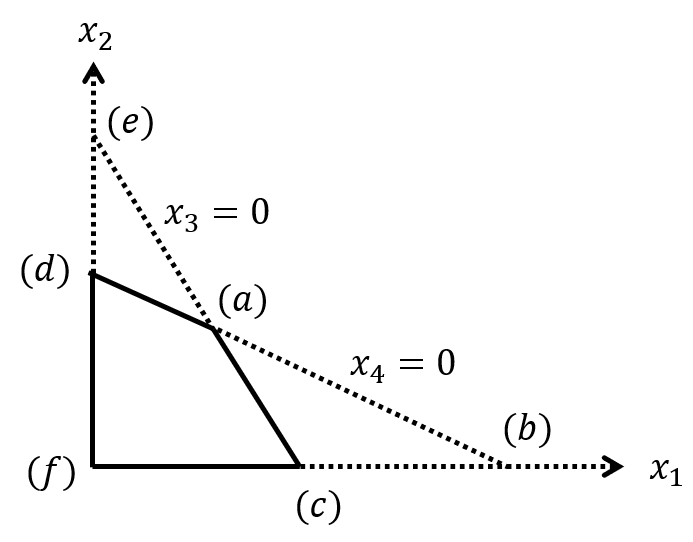
\includegraphics[width=7cm]{fig1.png}
\caption{式(2.6)もしくは式(2.7)の制約条件。実行可能解は実線で表された凸多面体に内包される。点$(a)-(f)$は式$(a)-(f)$の基底解に対応。}
\end{center}
\end{figure}
実行可能基底解の性質について議論するために、
\begin{equation}
\left\{
\begin{array}{l}
2x_1+x_2 \leq 6 \\
x_1 + 2x_2 \leq 6 \\
x_i \geq 0~(i=1,2)
\end{array}
\right.
\end{equation}
で表される制約条件を例題として扱おう。このときの実行可能解を図2.1に示す。これを標準形で書き換えると
\begin{equation}
\left\{
\begin{array}{l}
2x_1+x_2+x_3=6 \\
x_1+2x_2+x_4=6 \\
x_i \geq 0~(i=1,2,3,4)
\end{array}
\right.
\end{equation}
となる。この基底解は容易に求められ、
\begin{equation}
\begin{bmatrix}
x_1 & x_2 & x_3 & x_4
\end{bmatrix}=
\begin{bmatrix}
2 & 2 & 0 & 0
\end{bmatrix} \tag{a}
\end{equation}
\begin{equation}
\begin{bmatrix}
x_1 & x_2 & x_3 & x_4
\end{bmatrix}=
\begin{bmatrix}
6 & 0 & -6 & 0
\end{bmatrix} \tag{b}
\end{equation}
\begin{equation}
\begin{bmatrix}
x_1 & x_2 & x_3 & x_4
\end{bmatrix}=
\begin{bmatrix}
3 & 0 & 0 & 3
\end{bmatrix} \tag{c}
\end{equation}
\begin{equation}
\begin{bmatrix}
x_1 & x_2 & x_3 & x_4
\end{bmatrix}=
\begin{bmatrix}
0 & 3 & 3 & 0
\end{bmatrix} \tag{d}
\end{equation}
\begin{equation}
\begin{bmatrix}
x_1 & x_2 & x_3 & x_4
\end{bmatrix}=
\begin{bmatrix}
0 & 6 & 0 & -6
\end{bmatrix} \tag{e}
\end{equation}
\begin{equation}
\begin{bmatrix}
x_1 & x_2 & x_3 & x_4
\end{bmatrix}=
\begin{bmatrix}
0 & 0 & 6 & 6
\end{bmatrix} \tag{f}
\end{equation}
である。図2.1に示す通り、基底解は2本の直線が交わる点である。また、$(a)-(f)$のうち実行可能基底解は$(a)(c)(d)(f)$であり、これらは凸多面体の頂点である。\par
\begin{figure}[t]
\begin{center}
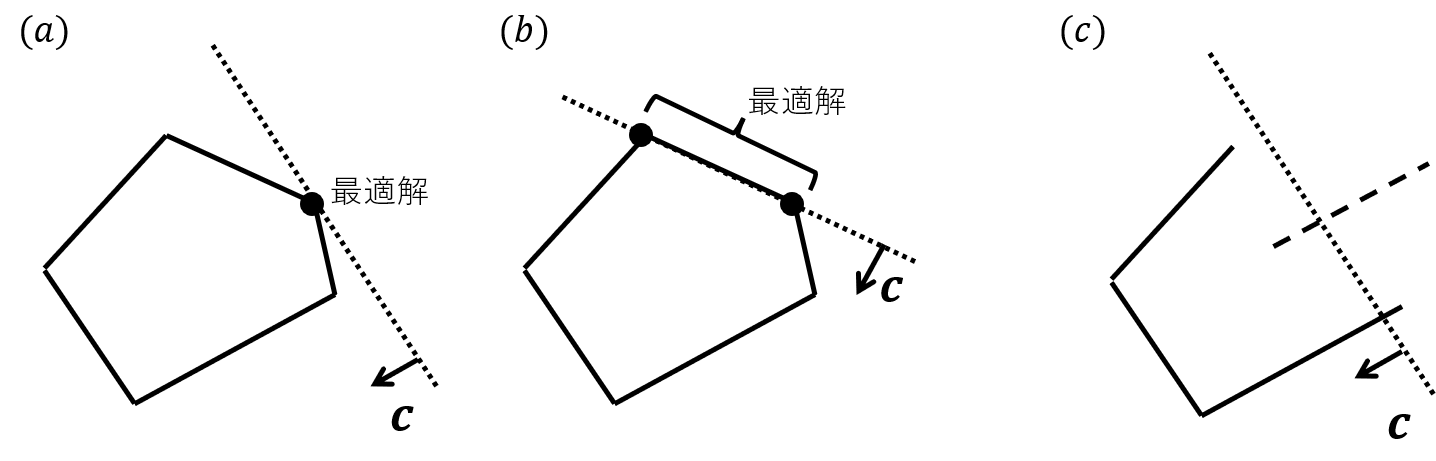
\includegraphics[width=12cm]{fig2.png}
\caption{線形計画問題の最適解。}
\end{center}
\end{figure}
さて、図2.2に示す通り目的関数の等高線は凸多面体に対する超平面になる。したがって線形計画問題の最適解について以下3つのことが言える。
\begin{itemize}
\item 図2.2(a)の場合、つまり最適値をとる目的関数と多面体が頂点で接するとき、ある1つの実行可能基底解が最適解となる。
\item 図2.2(b)の場合、つまり最適値をとる目的関数と多面体が面で接するとき、最適解は無数に存在する。ただしこのときも幾つかの実行可能基底解は最適解に含まれる。
\item 図2.2(c)の場合は最適解がなく、本節の議論の対象外である。
\item 図2.2に図持していないが、実行可能解が存在しない場合はこういった多面体が存在しない場合である。
\end{itemize}
\begin{itembox}[l]{定理2.1.2}
 線形計画問題が最適解を持つならば、実行可能基底解のなかに最適解が必ず存在する。
\end{itembox}

\subsubsection{シンプレックス法}
定理2.1.2より線形計画問題を見つける際は有限個の実行可能基底解を探索すればよいことが分かる。本節で紹介する{\bf シンプレックス法}は、より小さな目的関数値をもつ実行可能基底解を次々に生成し、最終的に最適基底解に到達しようとする反復法である。\par
そこで、標準形の問題に対して実行可能基底解を与える分割$\bm x=(\bm x_B~\bm x_N)^{\rm T}$並びに$A=(B~N)$が既に1つ与えられているとする(実行可能基底解を得る一般的な方法は後述する)。なお、あくまで実行可能基底解を与える分割が既知なだけで、$\bm x$は実行可能基底解でない。つまり、今は$\bm x_N \neq 0$である。$B$は正則なため、$\bm x_B$は式(2.5)より求まる。式(2.2)の目的関数について$\bm c$も$(\bm c_B~\bm c_N)^{\rm T}$のように分割したとき($\bm c_B \in \mathbb{R}^m$、$\bm c_N \in \mathbb{R}^{n-m}$)、目的関数値$z$は
\begin{equation}
z=\bm c_B^{\rm T}\bm x_B + \bm c_N^{\rm T}\bm x_N=\bm c_B^{\rm T}B^{-1}\bm b+(\bm c_N^{\rm T}-\bm c_B^{\rm T}B^{-1}N)\bm x_N=z_0+\sum_{j=m+1}^n(c_j-z_j)x_j
\end{equation}
となる。ここで
\begin{equation}
z_0=\bm c_B^{\rm T}B^{-1}\bm b,~~~z_j=\bm c_B^{\rm T}B^{-1}\bm a_j \notag
\end{equation}
であり、$\bm a_j$は$A$の第$j$列ベクトルである。$z_0$はこの分割における実行可能基底解$(\bm x_B~\bm 0)$に対する目的関数値である。式(2.8)より、$z$は$x_j$に対して$c_j-z_j$の感度で変化する。この$(c_j-z_j)$を$x_j$の{\bf 相対コスト係数}と言う。\par
分割$(\bm x_B~\bm x_N)^{\rm T}$および$(B~N)$に対して$j \in \{m+1,...,n\}$の相対コスト係数がいずれも非負である場合、$x_j \geq 0$並びに式(2.8)より$z \geq z_0$となる。従って全ての相対コスト係数が非負であるとき、この分割に対する実行可能基底解$\bm x=(B^{-1}\bm b~\bm 0)^{\rm T}$は最適解であり、最適値$z_0=\bm c_B^{\rm T}B^{-1}\bm b$	を返す。\par
一方で負の相対コスト係数$(c_p-z_p) < 0$となる$p \in \{m+1,...,n\}$が存在する場合を考える。$x_p$以外の$x_j \in \{m+1,...,n\}$をゼロとし、$x_p=\Delta(>0)$とする。このときの解
\begin{equation}
\bm x_{\Delta}=
\begin{bmatrix}
\bm x_b \\ x_{m+1} \\ . \\ . \\ . \\ x_p \\ . \\ .\\. \\ x_n
\end{bmatrix}
=\begin{bmatrix}
B^{-1}\bm b \\ 0 \\ . \\ . \\ . \\ \Delta \\ . \\ .\\. \\ 0
\end{bmatrix}
\end{equation}
に対する目的関数値は
\begin{equation}
\bm c^{\rm T}\bm x_{\Delta}=z_0+(c_p-z_p)\Delta \leq z_0
\end{equation}
となる。目的に従い目的関数は減少するため、実行可能基底解$(B^{-1}\bm b~\bm 0)^{\rm T}$から式(2.9)のような解の更新を考える。ただし、更新後も制約条件$A\bm x=\bm b$は満たされないといけないので、$\bm x_N$から$\bm x'_N=(0~0...\Delta...0)^{\rm T}$と変えたのならば、式(2.5)より$\bm x_B$も$\bm x_B=B^{-1}\bm b$から
\begin{equation}
\bm x'_B=B^{-1}\bm b-B^{-1}\bm a_p\Delta
\end{equation}
に変えなければならない。\par
また、$\bm x'_B \geq 0$でなければならないことも重要である。いま$B$は実行可能基底解を与えるような分割における基底行列であるため、$\bm x_B=B^{-1}\bm b\geq 0$である。一方で$B^{-1}\bm a_p \leq 0$の場合、任意の正の実数$\Delta$において式(2.11)の$\bm x_B'$は制約条件$\bm x_B' \geq 0$を満たす。式(2.10)より、$\Delta$の増加とともに目的関数値は減少するため、$\Delta$の値に上限がないならば目的関数値にも下限がないことになる。従って$B^{-1}\bm a_p \leq 0$なる$p$が存在する場合、この線形計画問題は有界な解を持たない。この判定は計算終了条件として重要である。\par
$p$に対して$(B^{-1}\bm a_p)_i > 0$となるような$i \in \{1, ..., m\}$が存在する場合、線形計画問題は有界な解を持たないとは限らない。$\Delta$の増加とともに目的関数値は減少することを思い出すと、式(2.11)の$\bm x_B'$が非負の制約条件を満たす最大の$\Delta$
\begin{equation}
\Delta={\rm min} \left\{ \frac{(B^{-1}\bm b)_i}{(B^{-1}\bm a_p)_i}|~(B^{-1}\bm a_p)_i>0~~i \in \{1, ..., m\} \right\}
\end{equation}
で解を更新すれば効率がよいと分かる。このとき新しい解$\bm x'$は
\begin{equation}
\bm x'=
\begin{bmatrix}
\bm x_B' \\ \bm x_N'
\end{bmatrix}
=
\begin{bmatrix}
B^{-1}\bm b - B^{-1}\bm a_p\Delta \\ 0 \\ . \\ .\\. \\ \Delta \\.\\.\\.\\0
\end{bmatrix}
\end{equation}
となる。$i=r(\in \{1, ..., m\})$のとき式(2.12)の右辺が最小となる場合、つまり$\Delta=(B^{-1}\bm b)_r/(B^{-1}\bm a_p)_i$である場合、式(2.13)の$x_r'$はゼロとなる。したがって$\bm x'$は少なくとも$n-m$個のゼロ要素を持つ。\par
シンプレックス法は次の解の更新時に、$n-m$個のゼロである変数が非基底変数となるように再度分割処理を施す。これは$r$番目の要素と$p$番目の要素を入れ替えるだけで済む。このとき$A$や$\bm c$の並び変えも必要であることに注意しなければならない($\bm b$は不要)。再分割により基底行列は$(\bm a_1~\bm a_2...\bm a_m)$から$(\bm a_1~\bm a_2...\bm a_{r-1}~\bm a_{p}~\bm a_{r+1}...\bm a_m)$に変わるが、再分割後の基底行列も正則であることは保証されている(証明は省く)。このような基底変数の入れ替えに伴う処理を{\bf ピボット演算}と言う。
以下にシンプレックス法のアルゴリズムを纏めた。
\begin{tcolorbox}[title=シンプレックス法]
 入力として実行可能基底解を与えるような分割が既に得られているとする。
\begin{enumerate}
\item $j \in \{m+1, ..., n\}$に対し相対コスト係数$c_j-z_j=c_j-\bm c_B^{\rm T}B^{-1}\bm a_j$を計算する。
\item 任意の$j$に対して$c_j-z_j \geq 0$ならば、$(B^{-1}\bm b~\bm 0)^{\rm T}$を最適解として出力し、計算を終了する。
\item 2.で計算が終了しなかった場合、$c_p-z_p < 0$となる$p \in \{m+1, ..., n\}$を一つ選択する。
\item $B^{-1}\bm a_p \leq \bm 0$の場合、この問題は有界な解を持たないと判断し、計算を終了する。
\item 4.で計算が終了しなかった場合、$\Delta \in \mathbb{R}$に${\rm min} \left\{ (B^{-1}\bm b)_i/(B^{-1}\bm a_p)_i|~(B^{-1}\bm a_p)_i>0~~i \in \{1, ..., m\} \right\}$を代入する。また、右辺について最小となる要素番号を$r \in \{1, ..., m\}$とする。
\item 解$\bm x=(B^{-1}\bm b~\bm 0)$を$\bm x'=(B^{-1}\bm b - B^{-1}\bm a_p\Delta~0...\Delta...0)^{\rm T}$に更新する(ここで$p$番目要素の値が$\Delta$)。
\item $\bm x'=(x'_1...x'_n)^{\rm T}$を$(x'_1...x'_{r-1}~x'_p~x'_{r+1}...x'_m~0...0)^{\rm T}$となるように入れ替える。
\item 7.に伴い$\bm c=(b_1...c_n)^{\rm T}$も$(c_1...c_{r-1}~c_p~c_{r+1}...c_{p-1}~c_r~c_{p+1}...c_n)^{\rm T}$となるように入れ替える。
\item 7.に伴い$A$も$(\bm a_1~\bm a_2...\bm a_n)$から$(\bm a_1...\bm a_{r-1}~\bm a_p~\bm a_{r+1}...\bm a_{p-1}~\bm a_r~\bm a_{p+1}...\bm a_n)^{\rm T}$となるように入れ替える。
\item $\bm x'$とピボット演算後の$A$を初期条件として、1.に戻る。
\end{enumerate}
\end{tcolorbox}\par
ピボット演算により変数の順番が変わるので、プログラム上ではそれを追跡する処理も必要となる。\par
シンプレックス法アルゴリズムの3.について、相対コスト係数が負であるならば$p$の選択は任意である。考え得る選択の一つとして、相対コスト係数が最小となる$p$を選択することである。つまり、
\begin{equation}
p={\rm argmin}\left\{ c_j-z_j|j \in \{m+1, ..., n\} \right\}
\end{equation}
となるように選択する。もちろん上式の最小値探査が計算コスト的に困難である場合は他の指針に従うべきであろう。

\subsubsection{理論的な収束性}
前述の通り、相対コスト係数$c_p-z_p$が負となる非基底変数$x_p$が見つかった場合、目的関数値は$|c_p-z_p|\Delta$だけ減少する。現段階の解$\bm x=(B^{-1}\bm b~\bm 0)^{\rm T}$に対して、制約条件より$B^{-1}\bm b \geq \bm 0$が成立する。そのため有界な解が存在する問題ならば、式(2.12)より$\Delta \geq 0$だと言える。とくに$B^{-1}\bm b>0$であるならば$\Delta>0$となり、解の更新によって目的関数値は狭義に減少する。線形計画問題の場合、解に対して目的関数値は一意に定まるので、シンプレックス法の反復計算中常に$B^{-1}\bm b>0$が成立するならば、更新されていく実行可能基底解の中に同一のものは存在しないはずである。実行可能基底解は有限個であることを思い出すと、このときシンプレックス法は有限回の反復計算で最適解に到達する。実行可能基底解$(\bm x_B~\bm x_N)^{\rm T}=(B^{-1}\bm b~\bm 0)^{\rm T}$が$B^{-1}\bm b>\bm 0$を満たすとき、この解のことを非退化であると言う。逆に非退化でない解のことを退化していると言う。

\begin{itembox}[l]{定理2.1.3}
 与えられた線形計画問題の初期実行可能基底解を求めることができ、しかも計算の途中に現れる実行可能基底解が全て非退化である場合、シンプレックス法は有限回の反復で最適解を見つける(もしくは有界な解がないことを識別して計算を終了する)。
\end{itembox}\par
退化の例として以下の問題を考える。
\begin{equation}
{\rm min}_{\bm x}~
\begin{bmatrix}
-3 & -2 & 0 & 0 & 0
\end{bmatrix}
\begin{bmatrix}
x_1 \\ x_2 \\ x_3 \\ x_4 \\ x_5
\end{bmatrix}~~~
{\rm s.t.}~~~
\begin{bmatrix}
2 & 1 & 1 & 0 & 0 \\
1 & 2 & 0 & 1 & 0 \\
1 & 0 & 0 & 0 & 1
\end{bmatrix}
\begin{bmatrix}
x_1 \\ x_2 \\ x_3 \\ x_4 \\ x_5
\end{bmatrix},~~\bm x \geq \bm 0.
\end{equation}
この問題の実行可能基底解として$\bm x_B=(x_1, x_2, x_4)^{\rm T}$、$\bm x_B=(x_1, x_3, x_4)^{\rm T}$、$\bm x_B=(x_1, x_4, x_5)^{\rm T}$が考えられるが、結局はいずれも$(3,0,0,4,0)^{\rm T}$であり、これは退化している。また、$(x_1, x_2)$-平面上で見たとき、この実行可能基底解は3本の直線の交わる点に対応している(図2.3の(3, 0))。\par
\begin{figure}[b]
\begin{center}
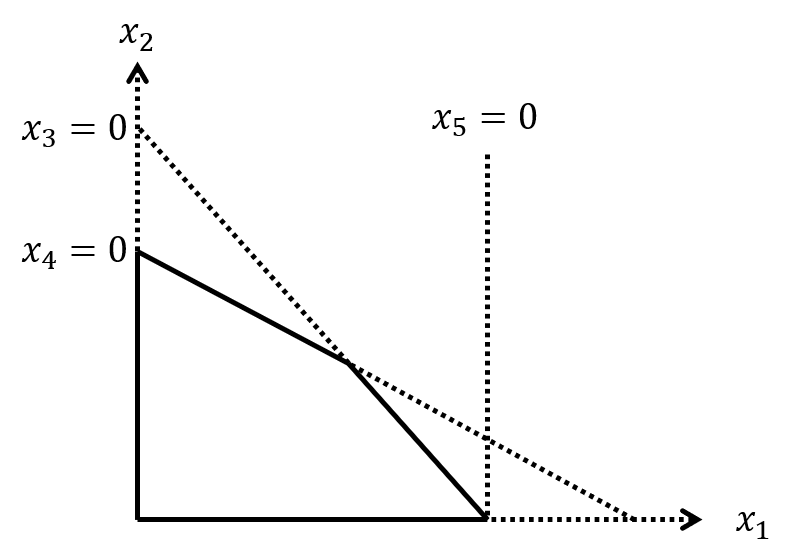
\includegraphics[width=7cm]{fig3.png}
\caption{式(2.15)の実行可能領域。}
\end{center}
\end{figure}
シンプレックス法の反復計算中に退化した実行可能基底解が現れると、式(2.12)の$\Delta$はゼロになる。そこでピボット演算をした場合、アルゴリズムの性質上基底変数と非基底変数の組み合わせは変わるが、解$\bm x$は実質的に動かず目的関数値も変化しない。また、基底に入る変数$p$が一意に定まらず、同時に基底から出る変数$r$も一意に定まらない場合、それらの選び方によっては何回かのピボット演算で同じ分割に戻ってしまう可能性もある。このような現象を{\bf 循環}と言う。循環が生じたときのシンプレックス法は同じ計算を何度も繰り返すことになり、最適解に到達できない。\par
循環という危険性を持っている点で、シンプレックス法は欠点のある手法と思われるかもしれない。ところが現実の問題で循環に出会うことはまずない。確かに退化が生じることは稀でないが、退化は循環の必要条件であって十分条件でなく、退化が生じたからと言って循環に神経質にならなくてもよい。\par
とはいえ運悪く循環が生じたときは困るので、いくつか循環を回避するための手法が研究された。その中でも最も有名なのが{\bf 最小添字規則}である。これは$p$や$r$の選択時、候補の中から最も添字小さいものを選ぶという規則であり。こうするだけでシンプレックス法は循環を確実に回避できる。ただし$p$の選択に関しては、前述の通り式(2.14)に従う選択の方が反復回数を抑えることができるので、最小添字規則がそのまま使われることは少ない。

\subsubsection{ビッグM法}
シンプレックス法は入力として実行可能基底解を与える分割を必要とする。これまでの問題では自明な実行可能基底解が存在したが、現実の問題で手計算によって実行可能基底解が得られることは稀であり、何か対策が必要である。本節ではプログラム実装が容易なビッグM法を紹介する。\par
ここで、対象の線形計画問題は既に標準形に変換されているとする。また$\bm b \geq 0$だと仮定する。仮に$b_i < 0$であったとしても、両辺に(-1)を掛ければよいため、この仮定は一般性を欠かない。ビッグM法では元の線形計画問題(2.3)の代わりに、
\begin{equation}
{\rm min}_{\bm (\bm x~\bm y)^{\rm T}}~\bm c^{\rm T}\bm x+M\bm d^{\rm T}\bm y~~~
{\rm s.t.}~~A\bm x+\bm y=\bm b,~~\bm x \geq 0,~~\bm y \geq 0
\end{equation}
を考える。ここで$\bm d \in \mathbb{R}^m$は全ての要素が1なベクトルで、$M\ in \mathbb{R}$はハイパーパラメータである。また$\bm y$は{\bf 人為変数}と言い、$\bm x$と同様に変数として考える。この線形計画問題は明らかに実行可能基底解$(\bm x~\bm y)^{\rm T}=(\bm 0~\bm b)^{\rm T}$を持つ。\par
$M$の値を十分に大きく設定した場合、目的関数に対して$M\bm d^{\rm T}\bm y$が支配的になり、シンプレックス法はまず第2項を減少させようと働く。その結果$\bm y=\bm 0$となれば、線形計画問題(2.16)は(2.3)と実質的に同じになる。従って、最終的に得られる解から$\bm x$に関わる要素を抽出すれば、所望の最適解が得られる訳である。\par
$M$の値が十分に大きくないとき、(2.16)の最適解に関して$\bm y=\bm 0$とならずに収束してしまうことがある。このときは$M$の値を更に大きくして再計算しなければならない。$M$を大きくし続けても$\bm y=\bm 0$とならずに収束するならば、元の問題(2.3)は実行可能解を持たないと判断し、計算を終了する。

\subsubsection{pythonコード例}
シンプレックス法の実装は数値計算の中だと比較的難しいと個人的に感じている。一方でシンプレックス法は研究しつくされた分野であり、既に多くのライブラリが開発されている。本節ではscipyを利用したコード例を紹介する。\par
扱う例題は
\begin{equation}
{\rm min}~-3x_1-2x_2~~~{\rm s.t.}~2x_1+x_2 \leq 6,~x_1+2x_2 \leq 6,~\bm x \geq 0 \notag
\end{equation}
とする。scipyのモジュールは前もって標準形に変換することも実行可能基底解を用意することも要求しない。上式の目的関数と制約条件を入力するだけで解が得られる仕様となっている。モジュールの使い方はscipyのマニュアルに譲り、本資料ではpythonコードを記すだけとした。

\begin{lstlisting}[caption=Pythonによるシンプレックス法コード例, language=Python]
import numpy as np
from scipy.optimize import linprog

c = np.array([-3., -2.])
Aub = np.array([
	[2., 1.],
	[1., 2.]])
bub = np.array([6.,6.])
bounds = np.array([0., None])
result = linprog(c, Aub, bub, bounds = bounds, method = "simplex")
x = result.x
\end{lstlisting}


\end{document}















\section{最適化手法}



\subsection{モーメント法と共役勾配法}
深層学習のように多数のパラメータを扱う場合、ヘッセ行列の数値計算は非現実的である。しかしながら、最急降下法は解更新における振動やあまりにもお粗末な局所解への収束などの問題を抱えている。そこで最急降下法の改良としてモーメント法が提案された。\par
モーメントは正に運動量のことであり、最適化手法におけるモーメント法は解の更新に慣性を持たせた手法と言える。最急降下法の場合、解は$\bm d_k=-\alpha \bm \nabla f(\bm x_k)$だけ更新していたが、モーメント法はこれを加味して
\begin{equation}
\bm d_k-\alpha \bm \nabla f(\bm x) + \beta \bm d_{k-1} \notag
\end{equation}
なる更新を施す。つまり、右辺第二項のように前回の更新値を足すことで慣性を与えている訳である。ここで$\beta$はハイパーパラメータで、0.9などの値を一般的に採用する。\par
モーメント法は深層学習の分野で提案された手法だが、それよりも前にあった共役勾配法と非常に似ている。共役勾配法では$\beta$をハイパーパラメータとせず、$f$の勾配から求める。求め方は4種類あり、それぞれ以下のように名付けられている。
\begin{itemize}
\item Fletcher-Reeves法:$\beta = || \bm \nabla f(\bm x_{k}) ||^2/|| \bm \nabla f(\bm x_{k-1}) ||^2$
\item Polak-Ribiere法:$\beta = \bm \nabla f(\bm x_{k})\cdot \bm y/|| \bm \nabla f(\bm x_{k-1}) ||^2$
\item Hestenes-Stiefel法:$\beta=\bm \nabla f(\bm x_{k})\cdot \bm y/(\bm d_{k-1}\cdot \bm y)$
\item Dai-Yuan法:$\beta=|| \bm \nabla f(\bm x_{k}) ||^2/(\bm d_{k-1}\cdot \bm y)$
\end{itemize}
ここで$\bm y=\bm \nabla f(\bm x_k)-\bm \nabla f(\bm x_{k-1})$である。この値にはきちんとした根拠があるが、本資料では触れない。

\subsection{AdaGrad}
AdaGradもヘッセ行列を必要としない手法であり、深層学習の分野で提案された。しかしハイパーパラメータに敏感なため、今ではあまり使われていない。\par
これまでに紹介した最急降下法やモーメント法では、勾配の反対方向に進み続ければ所望のパラメータに出会えると考えていた。それはテイラー展開ゆえに尤もなのだが、少し問題もある。例えば$\bm \nabla f(\bm x)$のうち、第$i$成分の値が大きくて第$j$成分の値が小さいとする。このとき$x_i$と比べて$x_j$の収束が遅れると想像できる。このようなギャップを抑えるためにAdaGradが提案された。\par
AdaGradでは更新幅$\bm d_k$を
\begin{equation}
d_{ki}=-\frac{\alpha}{\sum_{s=0}^{k} (\partial_if(\bm x_s))^2}\partial_if(\bm x_k) \notag
\end{equation}
に従い更新する。ここで$d_{ki}$はベクトル$\bm d_k$の第$i$成分である。第$i$成分において過去の勾配$\partial_if(\bm x_s)$の絶対値が大きかったなら、AdaGradは他と足並みを揃えるためにその後の更新を抑えるよう働く。しかしながら、これまでの勾配値がいつまでも影響を与えることはあまり良くない。例えば第$i$成分のパラメータにおいて、初め大きな勾配となる空間を探査してその後鞍点に入ったとする。解の更新的にはできるだけ早く鞍点から脱出したい訳だが、このとき初期の大きな勾配が邪魔をする。どうしても$d_{ki}$が小さな値となってしまうのである。最適化問題では、初めに非常に大きな勾配を取ることが多いので、この特徴は良くない。

\subsection{RMSprop}
AdaGradの改善のために、RMSpropでは十分過去の勾配の情報を指数的な減衰因子によって消滅させる。そのために、
\begin{equation}
v_{ki}=\rho v_{k-1i}+(1-\rho)(\partial_if(\bm x_k))^2
\end{equation}
\begin{equation}
d_{ki}=-\frac{\alpha}{v_{ki}+\epsilon}\partial_if(\bm x_k) \notag
\end{equation}
なる更新が行われる。ここで$\epsilon$は分母がゼロにならないためのハイパーパラメータであり、十分に小さな値を設定する。また$\rho$もハイパーパラメータであり、ゼロから1の値を設定する。$\rho$の値が大きくなるにつれ強い減衰となる。しかしながら、RMSpropも結果が学習率$\alpha$に敏感という問題を指摘されている。

\subsection{AdaDelta}
RMSpropの改良としてAdaDeltaが提案された。AdaDeltaでもRMSpropにおける式(1)のようなものを利用する。そこで、
\begin{equation}
\begin{array}{l}
{\rm RMS}(x_{ki})=\sqrt{v_{ki}+\epsilon} \\
v_{ki}=\rho v_{k-1i}+(1-\rho)x_{ki}^2
\end{array} \notag
\end{equation}
なるスカラー関数を定義しよう。このとき、AdaDeltaは
\begin{equation}
d_{ki}=-\frac{{\rm RMS}(d_{k-1i})}{{\rm RMS}(\partial_if(\bm x_k))}\partial_if(\bm x_k) \notag
\end{equation}
に従い更新する。

\subsection{Adam}
RMSpropの改良としてAdamが提案された。詳しくは議論しないが、AdamはRMSpropの式(1)の$v_{ki}$に加えて
\begin{equation}
m_{ki}=\rho'm_{k-1i}+(1-\rho)\partial_if(\bm x_k) \notag
\end{equation}
も利用する。ここで$\rho'$はハイパーパラメータであり、$\rho$と違う値であってもよい。さらにAdamでは、$v_{ki}$と$m_{ki}$を不偏推定量
\begin{equation}
\begin{array}{l}
\hat{v}_{ki}=v_{ki}/(1-\rho^k) \\
\hat{m}_{ki}=m_{ki}/(1-\rho'^k)
\end{array}\notag
\end{equation}
に変換する。最後に、
\begin{equation}
d_{ki}=-\frac{\alpha}{\sqrt{\hat{v}_{ki}+\epsilon}}\hat{m}_{ki} \notag
\end{equation}
に従い解を更新する。

\subsection{準ニュートン法}
2.3節から2.7節まで最急降下法の派生形のようなものを紹介してきたが、本節ではニュートン法の派生形として準ニュートン法を紹介する。準ニュートン法はヘッセ行列を近似し、目的関数の2解微分を回避した手法と言える。それゆえ準ニュートン法はニュートン法と比べて1回あたりの反復処理が速い。\par
準ニュートン法では、更新幅$\bm d_k$を$\bm d_k=-B_k^{-1}\bm \nabla f(\bm x_k)$もしくは$\bm d_k=-H_k\bm \nabla f(\bm x_k)$に従い決める。ニュートン法のアルゴリズムを見返せば、$B_k$はヘッセ行列の近似であること、並びに$H_k$はヘッセ行列の逆行列の近似であることが分かる。以下は準ニュートン法のアルゴリズムである。
\begin{tcolorbox}[title=準ニュートン法]
\begin{enumerate}
\item 初期解$\bm x_k \in \mathbb{R}^n$と$\alpha$、並びに$B_k$(もしくは$H_k$)を設定(ただし$k=0$)。$B_k(H_k)$の初期値として単位行列が考えられる。
\item $\bm x_k$が停止条件を満たす場合、$\bm x_k$を出力して終了。
\item $\bm d_k \leftarrow -\alpha B_k^{-1}\bm \nabla f(\bm x_k)$。もしくは$\bm d_k \leftarrow -\alpha H_k\bm \nabla f(\bm x_k)$
\item $\bm x_{k+1} \leftarrow \bm x_k + \bm d_k$。
\item $B_k(H_k)$を$B_{k+1}(H_{k+1})$に更新。
\item $k \leftarrow k+1$。ステップ2に戻る。
\end{enumerate}
\end{tcolorbox}
$B_k(H_k)$の候補としていくつか提案されているが、本資料ではBFGS公式を紹介する。BFGS公式では$B_k$もしくは$H_k$を以下のように更新する。
\begin{equation}
B_{k+1}=B_k-\frac{B_k\bm s_k\bm s_k^{\rm T}B_k}{\bm s_k^{\rm T}B_k\bm s_k}+\frac{\bm y_k\bm y_k^{\rm T}}{\bm s_k^{\rm T}\bm y_k} \notag
\end{equation}
\begin{equation}
H_{k+1}=\left(I-\frac{\bm s_k\bm y_k^{\rm T}}{\bm s_k^{\rm T} \bm y_k} \right)H_k
\left(I-\frac{\bm y_k\bm s_k^{\rm T}}{\bm s_k^{\rm T} \bm y_k} \right)+\frac{\bm s_k\bm s_k^{\rm T}}{\bm s_k^{\rm T} \bm y_k} \notag
\end{equation}
\begin{equation}
\bm s_k=\bm x_{k+1}-\bm x_k,~~~\bm y_k=\bm \nabla f(\bm x_{k+1})-\bm \nabla f(\bm x_k)
\end{equation}

\subsubsection{記憶制限付き準ニュートン法}
準ニュートン法によりヘッセ行列の計算は回避できたが、それでも$n\times n$行列を扱わなければならない。この行列の更新時に$O(n^2)$の計算が必要になるし、何より保存に要する計算メモリ量が痛い。そこで記憶制限付き準ニュートン法が提案された。BFGS公式を採用したときの記憶制限付き準ニュートン法は、よくL-BFGS法と略記される。L-BFGS法の計算量及び必要メモリ量は$O(mn)$まで削減できる。ここで$m$は自然数のハイパーパラメータであり、$n$と比べて非常に小さい。\par
L-BFGS法のアルゴリズムは準ニュートン法と同様だが、$\bm d_k$の計算方法だけ異なる。以下は$\bm d_k$の計算方法である。
\begin{tcolorbox}[title=L-BFGS法における更新幅計算]
\begin{enumerate}
\item 式(2)より、$\bm s_i, \bm y_i(i=k-1, k-2, ..., k-m)$を計算する。
\item $H_k \leftarrow (\bm s_{k-1}^{\rm T}\bm y_{k-1})/||\bm y_{k-1}||^2I$。
\item $\bm q \leftarrow \bm \nabla f(\bm x_k)$。
\item $i=k-1, ..., k-m$として、以下の5., 6.を反復。
\item $\tau_i \leftarrow (\bm s_i^{\rm T}\bm q)/(\bm s_i^{\rm T}\bm y_i)$。
\item $\bm q \leftarrow \bm q-\tau_i\bm y_i$。
\item $\bm d \leftarrow H_k\bm q$。
\item $i=k-m, k-m+1, ..., k-1$として以下の9.を反復。
\item $\bm d \leftarrow \bm d-(\bm y_i^{\rm T}\bm d)\bm s_i/(\bm s_i^{\rm T}\bm y_i)+\tau_i\bm s_i$。
\item $\bm d_k = -\alpha \bm d$を出力。
\end{enumerate}
\end{tcolorbox}


\end{document}












